\section{Causal Impact Analysis}
Before conducting our primary text mining analysis, we first establish the causal impact of ChatGPT on Stack Overflow question volumes. This section outlines our causal inference methodology and findings, which provide critical context for interpreting the subsequent textual analysis results.

%%%%%%%%%%%%%%%%%%%%%%%%%%%%%%%%%%%%%%%%%%%%%%%%%%%%%%%%%%%%%%%%%%%%%%%%%%%%%%%%%%%%%%%%%%%%%%%%

\subsection{Synthetic Difference-in-Differences Methodology}
To identify the causal impact of ChatGPT on Stack Overflow question volumes, we employ a Synthetic Difference-in-Differences (SDID) approach (\cite{arkhangelsky_synthetic_2021}). This methodology combines the strengths of traditional difference-in-differences and synthetic control methods, allowing us to construct a credible counterfactual for Stack Overflow in the absence of ChatGPT.\\

The selection of Mathematics, Physics, Superuser, and AskUbuntu as control units was strategically motivated by several considerations. First, these Stack Exchange forums represent technical knowledge domains with structured question patterns similar to Stack Overflow, yet they address distinct subject matters that were less effectively handled by early ChatGPT versions. While ChatGPT demonstrated strong capabilities in programming tasks from its initial release, it exhibited notable limitations in advanced mathematics, physics reasoning, and system-specific troubleshooting—areas central to our control forums. Second, these forums maintain sufficient question volumes to provide statistical power while exhibiting pre-treatment correlation with Stack Overflow question patterns (cf. \figureref{fig:correlation_matrix}), suggesting similar responsiveness to seasonal trends and external factors affecting forum usage.\\

A critical assumption for traditional difference-in-differences analysis is the parallel trends assumption, which requires that treatment and control groups would follow similar trajectories in the absence of treatment. While examining raw counts shows substantial scale differences between forums, log transformation reveals approximately parallel pre-treatment trends, particularly for scripting language questions (cf. Figure \ref{fig:paralleL_trend_trans}). This transformation addresses heterogeneity in question volumes and improves the validity of our causal inference by better satisfying the parallel trends assumption.\\

\begin{figure}[H]
    \centering
    \includesvg[width=1\linewidth]{imgs/transformed_trends.svg}
    \caption{Parallel trends: Weekly raw vs logged question scripting question counts}
    \label{fig:paralleL_trend_trans}
\end{figure}

Despite the similar pre-treatment trends, concerns remain about external shocks that might differentially affect Stack Overflow and control forums. Our methodological approach addresses this in two complementary ways. First, our baseline DiD implementation using Stata's \mintinline{stata}{xtdidregress} automatically adjusts for both panel (forum) effects and time effects in calculating the treatment effect. We verified the robustness of these results by explicitly testing specifications with additional time fixed effects at various granularities (weekly, monthly, quarterly), which yielded identical treatment effect estimates.\\

Second, our synthetic DiD approach further strengthens causal identification by constructing a weighted combination of control units that better approximates the counterfactual for Stack Overflow. This method implicitly accounts for time-varying factors to the extent they similarly affect both treatment and control units, creating a more credible counterfactual than standard DiD approaches relying solely on parallel trends assumptions. Together, these approaches provide robust evidence that our findings reflect the causal impact of ChatGPT rather than coincidental time-specific shocks.

%%%%%%%%%%%%%%%%%%%%%%%%%%%%%%%%%%%%%%%%%%%%%%%%%%%%%%%%%%%%%%%%%%%%%%%%%%%%%%%%%%%%%%%%%%%%%%%%

\subsubsection{Model Specification}
Our base difference-in-differences (DiD) model can be expressed as:

\begin{equation}\label{eq:basedid}
\ln(Q_{it}) = \beta_1(Treatment_i \times Post_t) + \gamma_i + \lambda_t + \varepsilon_{it}
\end{equation}

where $\ln(Q_{it})$ represents the log-transformed question count for forum $i$ at time $t$, $\text{Treatment}_i$ is an indicator for Stack Overflow (being 1 in the case of Stack Overflow and 0 otherwise), $\text{Post}_t$ is an indicator for periods after ChatGPT's release (November 30, 2022, being 1 after and 0 otherwise).  Furthermore, $\gamma_i$ represents forum fixed effects, $\lambda_t$ represents time fixed effects, and $\varepsilon_{it}$ is the error term. Lastly, the coefficient $\beta_1$ captures the average treatment effect on the treated (ATET) - the causal impact of ChatGPT on Stack Overflow question volume.\\

For our synthetic DiD approach, we follow \textcite{arkhangelsky_synthetic_2021}, where the estimator can be expressed as:

\begin{equation}\label{eq:synthdid}
\hat{\tau}_{\text{SDID}} = \sum_{t=T_0+1}^T \lambda_t \left( Y_{1t} - \sum_{j=2}^J \omega_j Y_{jt} \right) - \sum_{t=1}^{T_0} \lambda_t \left( Y_{1t} - \sum_{j=2}^J \omega_j Y_{jt} \right)
\end{equation}

where $Y_{jt}$ represents the log-transformed question count for forum $j$ at time $t$, $\omega_j$ are unit weights, $\lambda_t$ are time weights, $T_0$ is the last pre-treatment period, and unit $j=1$ represents Stack Overflow. We implemented this methodology using \textcite{clarke_synthetic_2023, ciccia_short_2024}'s Stata implementation to ensure robustness of our findings, and conducted both static SDID analysis and dynamic event study specifications.

%%%%%%%%%%%%%%%%%%%%%%%%%%%%%%%%%%%%%%%%%%%%%%%%%%%%%%%%%%%%%%%%%%%%%%%%%%%%%%%%%%%%%%%%%%%%%%%%

\subsection{Causal Impact Results}

%%%%%%%%%%%%%%%%%%%%%%%%%%%%%%%%%%%%%%%%%%%%%%%%%%%%%%%%%%%%%%%%%%%%%%%%%%%%%%%%%%%%%%%%%%%%%%%%

\subsubsection{Base DiD Estimates}
We begin with standard DiD estimates for both all Stack Overflow questions and specifically for scripting language questions (JavaScript, Python, R, and PHP). Table \ref{tab:did_results} presents these results.

\begin{table}[H]
    \centering
    \caption{DiD Estimates of ChatGPT's Impact on Stack Overflow Question Volume}
    \label{tab:did_results}
    \begin{tabular}{lcc}
        \toprule
            & \multicolumn{2}{c}{Log Question Count (\equationref{eq:basedid})} \\
            \cmidrule(lr){2-3}
            & All Questions & Scripting Languages \\
        \midrule
            Treatment Effect & $-0.241^{***}$ & $-0.457^{***}$ \\
            & $(0.034)$ & $(0.034)$ \\
        \midrule
            Time FE & Yes & Yes \\
            Observations & 830 & 830 \\
        \bottomrule
            \multicolumn{3}{l}{\footnotesize Standard errors clustered by forum in parentheses} \\
            \multicolumn{3}{l}{\footnotesize $^{*}p<0.05$, $^{**}p<0.01$, $^{***}p<0.001$} \\
    \end{tabular}
\end{table}

These results indicate statistically significant negative effects, with a larger magnitude for scripting language questions. Specifically, while the overall Stack Overflow question volume decreased by approximately 21.4\% ($e^{-0.241}-1$), scripting language questions saw a much larger decline of 36.7\% ($e^{-0.457}-1$). This differential impact suggests that ChatGPT has been particularly effective at addressing programming questions related to these popular scripting languages.

%%%%%%%%%%%%%%%%%%%%%%%%%%%%%%%%%%%%%%%%%%%%%%%%%%%%%%%%%%%%%%%%%%%%%%%%%%%%%%%%%%%%%%%%%%%%%%%%

\subsubsection{Synthetic DiD Results}
To address potential violations of the parallel trends assumption and create a more credible counterfactual, we employ the SDID approach. Figure \ref{fig:sdid_all} visualizes the results for all Stack Overflow questions, while Figure \ref{fig:sdid_script} focuses on scripting language questions, and Table \ref{tab:sdid_results} presents the formal SDID estimates.

\begin{figure}[H]
    \centering
    \begin{subfigure}[b]{0.475\textwidth}
        \centering
        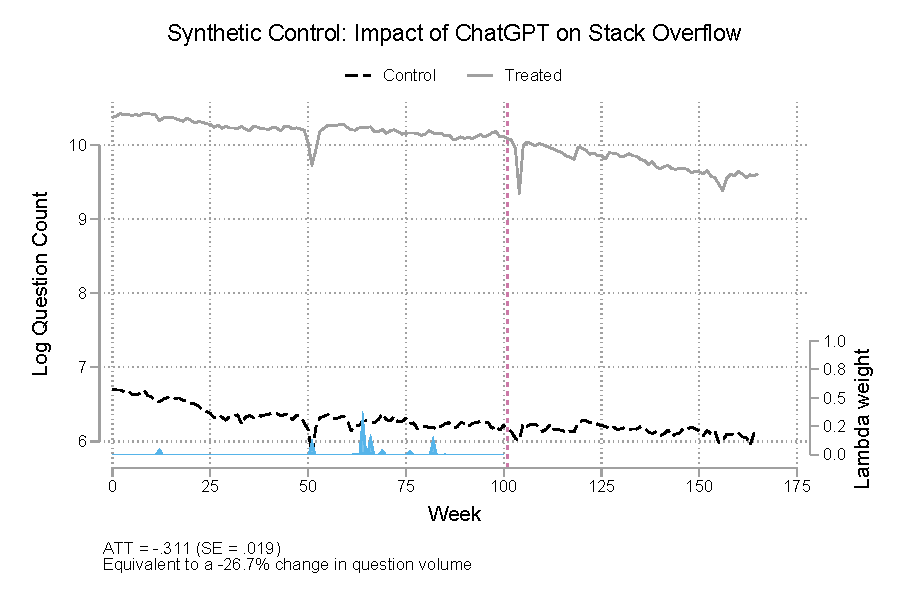
\includegraphics[width=1\textwidth]{imgs/stata/sdid_all_trends101.pdf}
        \caption{Impact on All Stack Overflow Questions}
        \label{fig:sdid_all}
    \end{subfigure}
    \hfill
    \begin{subfigure}[b]{0.475\textwidth}
        \centering
        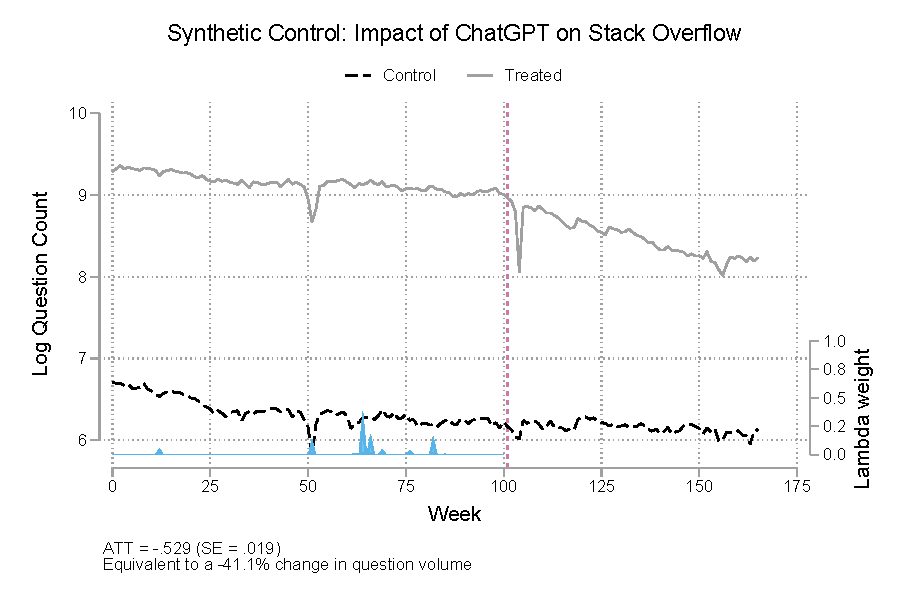
\includegraphics[width=1\textwidth]{imgs/stata/sdid_script_trends101.pdf}
        \caption{Impact on Scripting Language Questions}
        \label{fig:sdid_script}
    \end{subfigure}
    \caption{Synthetic difference-in-difference plots}
    \label{fig:DiD}
\end{figure}

\begin{table}[H]
    \centering
    \caption{Synthetic DiD Estimates of ChatGPT's Impact on Stack Overflow}
    \label{tab:sdid_results}
    \begin{tabular}{lcc}
        \toprule
            & \multicolumn{2}{c}{Log Question Count (\equationref{eq:synthdid})} \\
            \cmidrule(lr){2-3}
            & All Questions & Scripting Languages \\
        \midrule
            Average Treatment Effect & $-0.311^{***}$ & $-0.529^{***}$ \\
            & $(0.019)$      & $(0.019)$ \\
            \midrule
            Percent Change & $-26.7\%$ & $-41.1\%$ \\
            Observations & 830 & 830 \\
        \bottomrule
            \multicolumn{3}{l}{\footnotesize Standard errors based on placebo replications} \\
            \multicolumn{3}{l}{\footnotesize $^{*}p<0.05$, $^{**}p<0.01$, $^{***}p<0.001$} \\
    \end{tabular}
\end{table}

The SDID approach yields larger treatment effect estimates compared to standard DiD, suggesting that the traditional DiD may underestimate the impact. The SDID results indicate a 26.7\% reduction in overall question volume and a substantial 41.1\% reduction in scripting language questions.

%%%%%%%%%%%%%%%%%%%%%%%%%%%%%%%%%%%%%%%%%%%%%%%%%%%%%%%%%%%%%%%%%%%%%%%%%%%%%%%%%%%%%%%%%%%%%%%%

\subsubsection{Event Study Analysis}
We conducted a synthetic event study analysis to explore how the treatment effect evolved over time, following \textcite{ciccia_short_2024}:

\begin{equation}
    \ln(Q_{it}) = \sum_{k=-K}^{K'} \beta_k (Treatment_i \times D_{t,k}) + \gamma_i + \lambda_t + \varepsilon_{it}
\end{equation}

Where: $\ln(Q_{it})$ is the log-transformed question count for forum $i$ at time $t$, $Treatment_i$ is the indicator for Stack Overflow (1 for Stack Overflow, 0 otherwise),  $D_{t,k}$ are indicators for being $k$ periods away from the treatment date. Moreover, $K$ is the maximum number of periods before treatment included in the model and $K'$ is the maximum number of periods after treatment included in the model. Lastly, $\gamma_i$ represents forum fixed effects, $\lambda_t$ represents time fixed effects, $\varepsilon_{it}$ is the generic error term.\\

The coefficients $\beta_k$ represent the treatment effect $k$ periods away from the ChatGPT release date, with $k < 0$ for pre-treatment periods and $k > 0$ for post-treatment periods. Typically, one pre-treatment period (often $k = -1$) is omitted as the reference period, normalizing the effect to zero at that point. When implemented in the synthetic DiD framework, each coefficient $\beta_k$ is estimated using the synthetic control method, comparing Stack Overflow to a weighted combination of control forums optimized for that specific time period. Figure \ref{fig:event_study} displays the results for scripting language questions.

\begin{figure}[H]
    \centering
    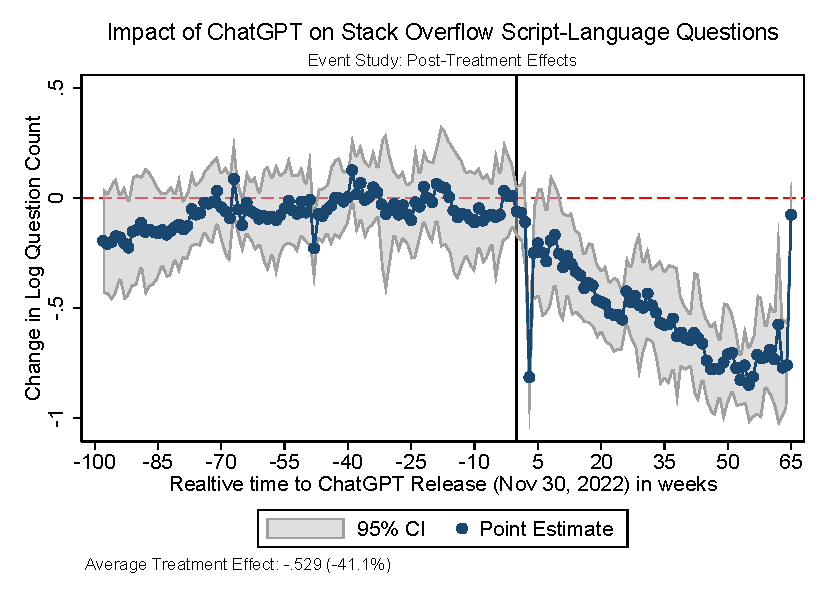
\includegraphics[width=1\textwidth]{imgs/stata/event_study_scripting_languages.pdf}
    \caption{Event Study Analysis for Scripting Language Questions}
    \label{fig:event_study}
\end{figure}

The event study reveals several important patterns: (1) The pre-treatment coefficients (points to the left of time 0) are clearly not centered exactly at zero. There appears to be a slight negative trend in the pre-treatment period, with most estimates falling between -0.2 and -0.1. However, most pre-treatment point estimates have confidence intervals that include zero (particularly in the periods closer to treatment). (2) An immediate and substantial drop in question volume following ChatGPT's release. (3) Persistence of the effect throughout the post-treatment period. (4) Slight intensification of the effect over time, suggesting continued adoption of ChatGPT for programming assistance.

%%%%%%%%%%%%%%%%%%%%%%%%%%%%%%%%%%%%%%%%%%%%%%%%%%%%%%%%%%%%%%%%%%%%%%%%%%%%%%%%%%%%%%%%%%%%%%%%

\subsection{Robustness and Potential Confounders}

The stability of our DiD estimates across different time fixed effect specifications provides evidence of robustness. However, we must acknowledge potential confounders that could threaten causal identification:

\begin{enumerate}
    \item \textbf{Concurrent AI releases:} The period following ChatGPT's release saw the introduction of other AI models and tools. While these likely had smaller impacts than ChatGPT given its widespread adoption, they could contribute to the observed effects. Our time fixed effects partially address this by controlling for common temporal shocks.
    \item \textbf{Forum-specific trends:} Although we control for time-invariant forum characteristics and common time shocks, forum-specific trends could potentially confound our results. The synthetic control approach helps mitigate this concern by creating a weighted combination of control units that better approximates the counterfactual.
    \item \textbf{Spillover effects:} Users might have reduced their activity across multiple Stack Exchange forums after discovering ChatGPT, creating spillover effects that could attenuate our estimates. If present, this would mean our results are conservative.
\end{enumerate}

Despite these considerations, the effects' magnitude, immediacy, and persistence, particularly for scripting languages, strongly suggest a causal relationship between ChatGPT's introduction and the observed decline in Stack Overflow question volume.

%%%%%%%%%%%%%%%%%%%%%%%%%%%%%%%%%%%%%%%%%%%%%%%%%%%%%%%%%%%%%%%%%%%%%%%%%%%%%%%%%%%%%%%%%%%%%%%%

\subsection{Implications for Text Analysis}

These findings establish a causal impact of ChatGPT on Stack Overflow question volumes, particularly for scripting language questions. The differential impact on scripting languages (41.1\% reduction compared to 26.7\% overall) suggests that ChatGPT has been particularly effective at addressing common programming queries.

This causal foundation motivates our core research question: How has the nature of the remaining questions changed? The dramatic reduction in volume indicates a fundamental shift in how developers seek programming assistance. Still, it raises important questions about the characteristics of questions that continue to be asked on Stack Overflow despite the availability of ChatGPT. Our subsequent text mining analysis will identify and quantify these changes in question content, complexity, and topical focus.